\chapter{Регионы России}
\label{ch:oblast-of-Russia}
%
\label{question:q_subjects_of_Russia_3}
\marginnote[0.6\baselineskip]{О флаге какого региона идёт речь:
<<Флаг этого субъекта представляет собой прямоугольное полотнище с отношением ширины к длине 2:3, 
красного цвета с двусторонним изображением в верхнем 
ближнем к древку углу основного элемента герба этого субъекта~--- 
развёрнутого к древку Святого \href{https://ru.wikipedia.org/?curid=151255}{Георгия Победоносца}.\\ \\
См. ответ \ref{answer:subjects_of_Russia_3} на с.~\pageref{answer:subjects_of_Russia_3}.%
}


Эта глава посвящена исследованию в Викиданных регионов России. 
Отметим, что регионы России включают в себя множество земель разного 
типа: области, республики, края и другие. Именно эти разнотипные регионы 
и были исследованы. 
Был построен граф субъектов России, граничащих с зарубежными странами (граф соседей), 
а также нарисована карта, 
на которой отмечена численность населения отдельных регионов. 
Оценка степени заполненности свойства Викиданных <<граничит с>> (shares border with) 
показала, что у~каждого субъекта России эти данные заполнены полностью. 
Были построены две карты, на которых цветом обозначены граничные регионы и пограничные страны.
Читатель познакомится с компьютерной обработкой Викиданных и визуализацией 
информации о регионах России.


\section{Экземпляры объекта <<Области России>>}

Для построения списка всех областей России нам потребуются объект 
\wdqName{<<области России>>}{835714} и свойство \wdProperty{31}{<<экземпляры>>} 
(листинг~\ref{lst:oblast-of-Russia}).


\begin{marginfigure}[-5\baselineskip]
\begin{lstlisting}[ language=SPARQL, numbers=none,
                    caption={\href{https://w.wiki/4D2V}{Список всех областей России}},
                    label=lst:oblast-of-Russia,
                    numbers=none,
                    texcl 
                    ]
# List of regions of Russia
SELECT ?region ?regionLabel WHERE
{
  ?region wdt:P31 wd:Q835714. # is "oblast of Russia"
  SERVICE wikibase:label { bd:serviceParam 
                           wikibase:language "ru" }
}
\end{lstlisting}%
Получено 48 записей в 2017 году и 46 записей в 2021 году. Ссылка на~SPARQL-запрос: \href{https://w.wiki/4D2V}{https://w.wiki/4D2V}.\\
\end{marginfigure}


В Викиданных больше всего свойств в России и в мире у \wdqName{Ленинградской}{2191} 
и~\wdqName{Калининградской областей}{1749}, по 43 свойства\autocite{Russia_prowd}. 
Число свойств у этих областей для России и мира одинаковое, так как и для России, и для мира это одни и те же объекты.

Областями России с наименьшим числом свойств по данным сервиса ProWD оказались: 
\href{http://www.wikidata.org/entity/Q3129}{Орловская} и \href{http://www.wikidata.org/entity/Q3178}{Курская} области (по 31 свойству) и \href{http://www.wikidata.org/entity/Q5851}{Новосибирская область} (32 свойства).




\section{Субъекты Российской Федерации}

Построим список всех субъектов России. 
Для этого выберем следующие объекты в Викиданных: 
республики, края, области, города федерального значения, автономные области и~автономные округа (листинг~\ref{lst:subjects-of-Russia}).

%\footnotetext{
\marginnote{Используемые в запросах объекты:
\begin{itemize}
	\item\wdqName{<<области России>>}{835714};
	\item\wdqName{<<республики России>>}{41162};
	\item\wdqName{<<города федерального значения России>>}{183342};
	\item\wdqName{<<края России>>}{831740};
	\item\wdqName{<<автономные области России>>}{309166};
	\item\wdqName{<<автономные округа России>>}{184122};
	\item\wdqName{<<бывшая административно-территориальная единица>>}{19953632}.
\end{itemize}
Используемое свойство~--- \wdProperty{31}{<<экземпляры>>}
}

\begin{lstlisting}[ language=SPARQL, numbers=none,
                    caption={\href{https://w.wiki/4D2R}{Список всех субъектов России}\protect\footnotemark},
                    label=lst:subjects-of-Russia,
                    texcl 
                    ]
# List of `instances of` "subjects of Russia" 
SELECT ?subject ?subjectLabel ?typeLabel WHERE
{  
  VALUES ?type {wd:Q835714   # oblast of Russia
                wd:Q41162    # republic of Russia
                wd:Q183342   # federal city of Russia
                wd:Q831740   # krai of Russia
                wd:Q309166   # autonomus oblast of Russia
                wd:Q184122}  # autonomus okrug of Russia
  ?subject wdt:P31 ?type.  # selecting the type of object
  SERVICE wikibase:label { bd:serviceParam wikibase:language "ru" }
}
\end{lstlisting}%
\footnotetext{Получено 85 записей в 2017 году и 86 записей в 2021 году. Ссылка на~SPARQL-запрос: \href{https://w.wiki/4D2R}{https://w.wiki/4D2R}. В 2021 году в список субъектов добавился город федерального значения Байконур на правах аренды комплекса <<Байконур>>.}

Для построения скрипта~\ref{lst:subjects-of-Russia} и проверки результатов учтём следующую информацию:
\begin{itemize}
  \item По данным Конституции Российской Федерации Россия состоит из 85 субъектов~--- республик, краёв, областей, городов федерального значения, автономной области, автономных округов.
  \item При построении списка объектов не нужно в него включать такие субъекты, 
      которые на~текущий момент не входят в состав РФ (например, \wdqName{Читинская область}{182902}). 
      Такие объекты легко отсеить, поскольку 
        они не являются экземплярами объектов \wdqName{<<области России>>}{835714}, 
        \wdqName{<<республики России>>}{41162}, 
        \wdqName{<<города федерального значения России>>}{183342}, 
        \wdqName{<<края России>>}{831740}, 
        \wdqName{<<автономные области России>>}{309166}, 
        \wdqName{<<автономные округа России>>}{184122}, 
      а~относятся к~объекту \wdqName{<<бывшая административно-территориальная единица>>}{19953632}. 
  \item В статье Русской Википедии <<\href{https://ru.wikipedia.org/?curid=1042}{Субъекты Российской Федерации}>> 
        и в статье Английской Википедии ``\href{https://en.wikipedia.org/wiki/Federal_subjects_of_Russia}{Federal subjects of Russia}'' 
        перечислено по 85 субъектов РФ.
\end{itemize}





\section{Соседние субъекты}

Построим граф соседних субъектов России, используя свойство \wdProperty{47}{shares border with}, 
с помощью запроса~\ref{lst:sharesBorderWith-oblast-of-Russia}.

\label{question:q_subjects_of_Russia_1}
\marginnote[-1\baselineskip]{Назовите регион России, 
расположенный на~северо-западе России 
и~образованный в \num{1920} году. 
Он граничит с Ленинградской, Вологодской, Архангельской и Мурманской областью. 
Также граничит с Финляндией на~западе.
Выберите среди следующих флагов флаг этого региона.\\ \\
См. ответ \ref{answer:subjects_of_Russia_1} на с.~\pageref{answer:subjects_of_Russia_1}.}
\begin{marginfigure}[0.0cm]
\centering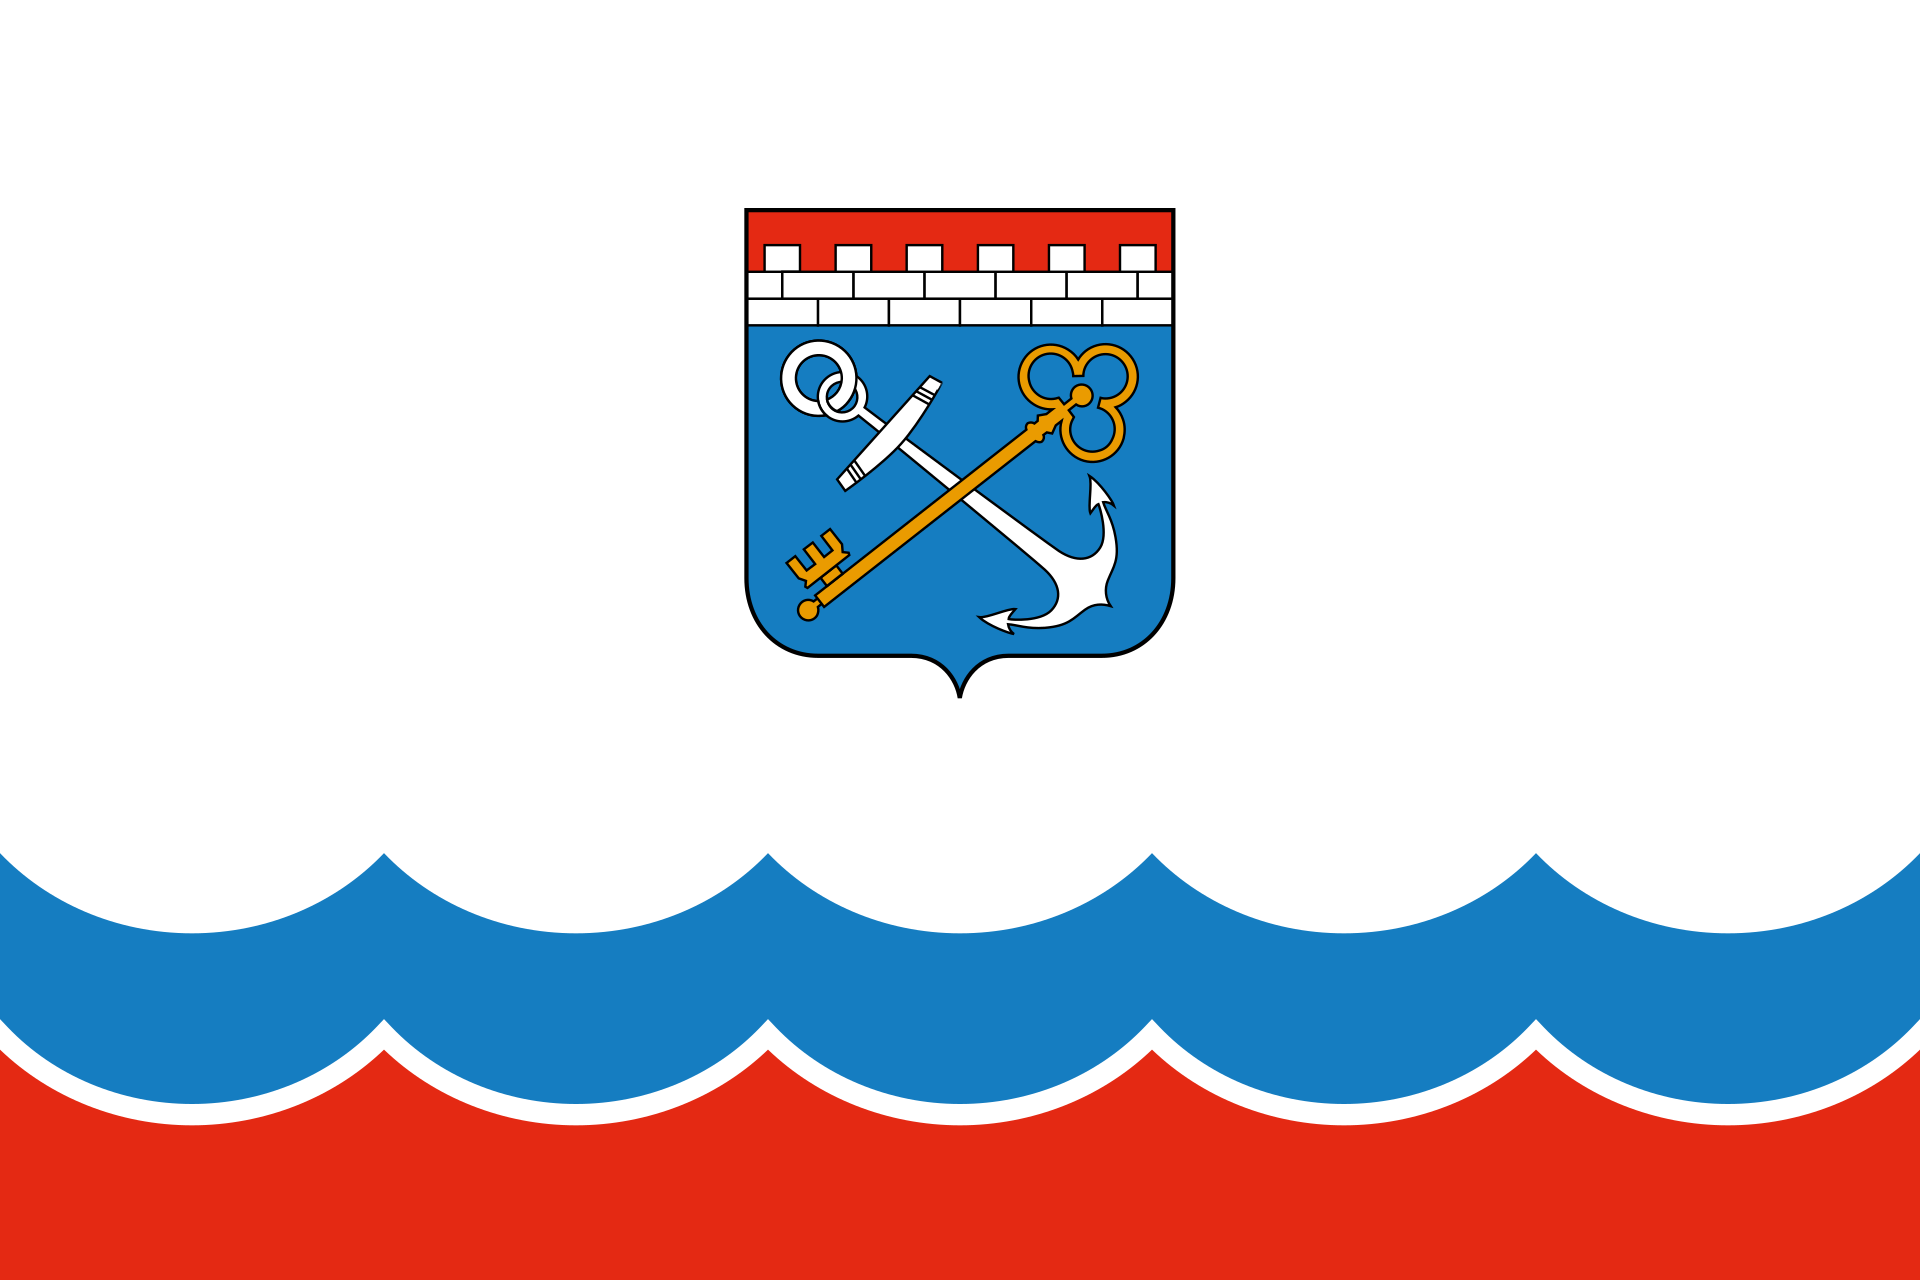
\includegraphics[width=3cm]{"chapter/oblast_of_Russia/Flag_of_Leningrad_Oblast.png"}
\caption [Флаг Ленинградской области.]{Флаг Ленинградской области.}%
\label{fig:Flag_of_Leningrad_Oblast}%
\end{marginfigure}

\begin{marginfigure}[0.0cm]
\centering
\includegraphics[width=3cm]{"chapter/oblast_of_Russia/Flag_of_Moscow_oblast.png"}
\caption [Флаг Московской области.]{Флаг Московской области.}%
\label{fig:Flag_of_Moscow_oblast}%
\end{marginfigure}

\begin{marginfigure}[0.0cm]
\centering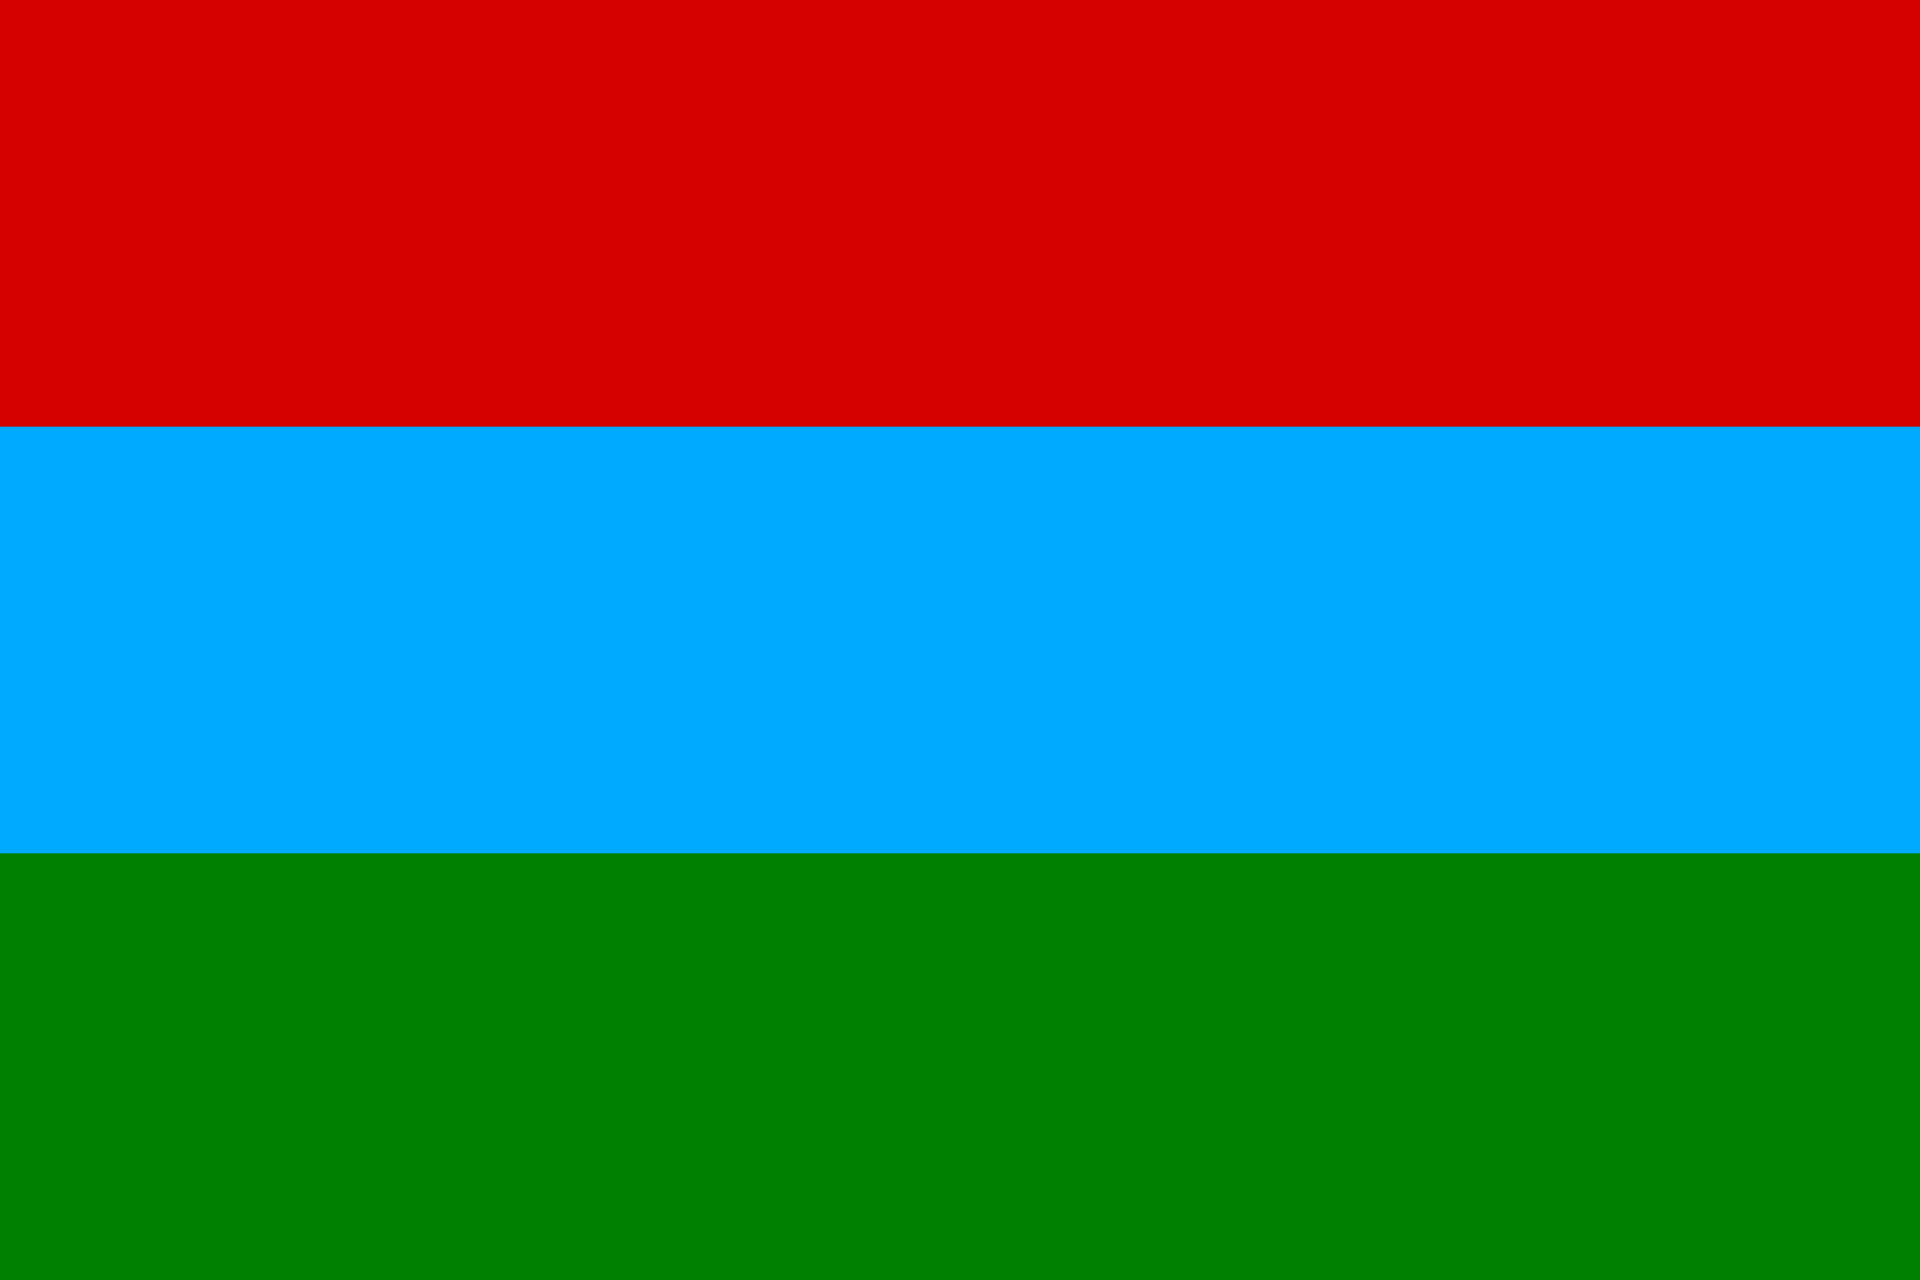
\includegraphics[width=3cm]{"chapter/oblast_of_Russia/Flag_of_Karelia.png"}
\caption [Флаг Карелии.]{Флаг Карелии.}%
\label{fig:Flag_of_Karelia}%
\end{marginfigure}

\begin{marginfigure}[0.0cm]
\centering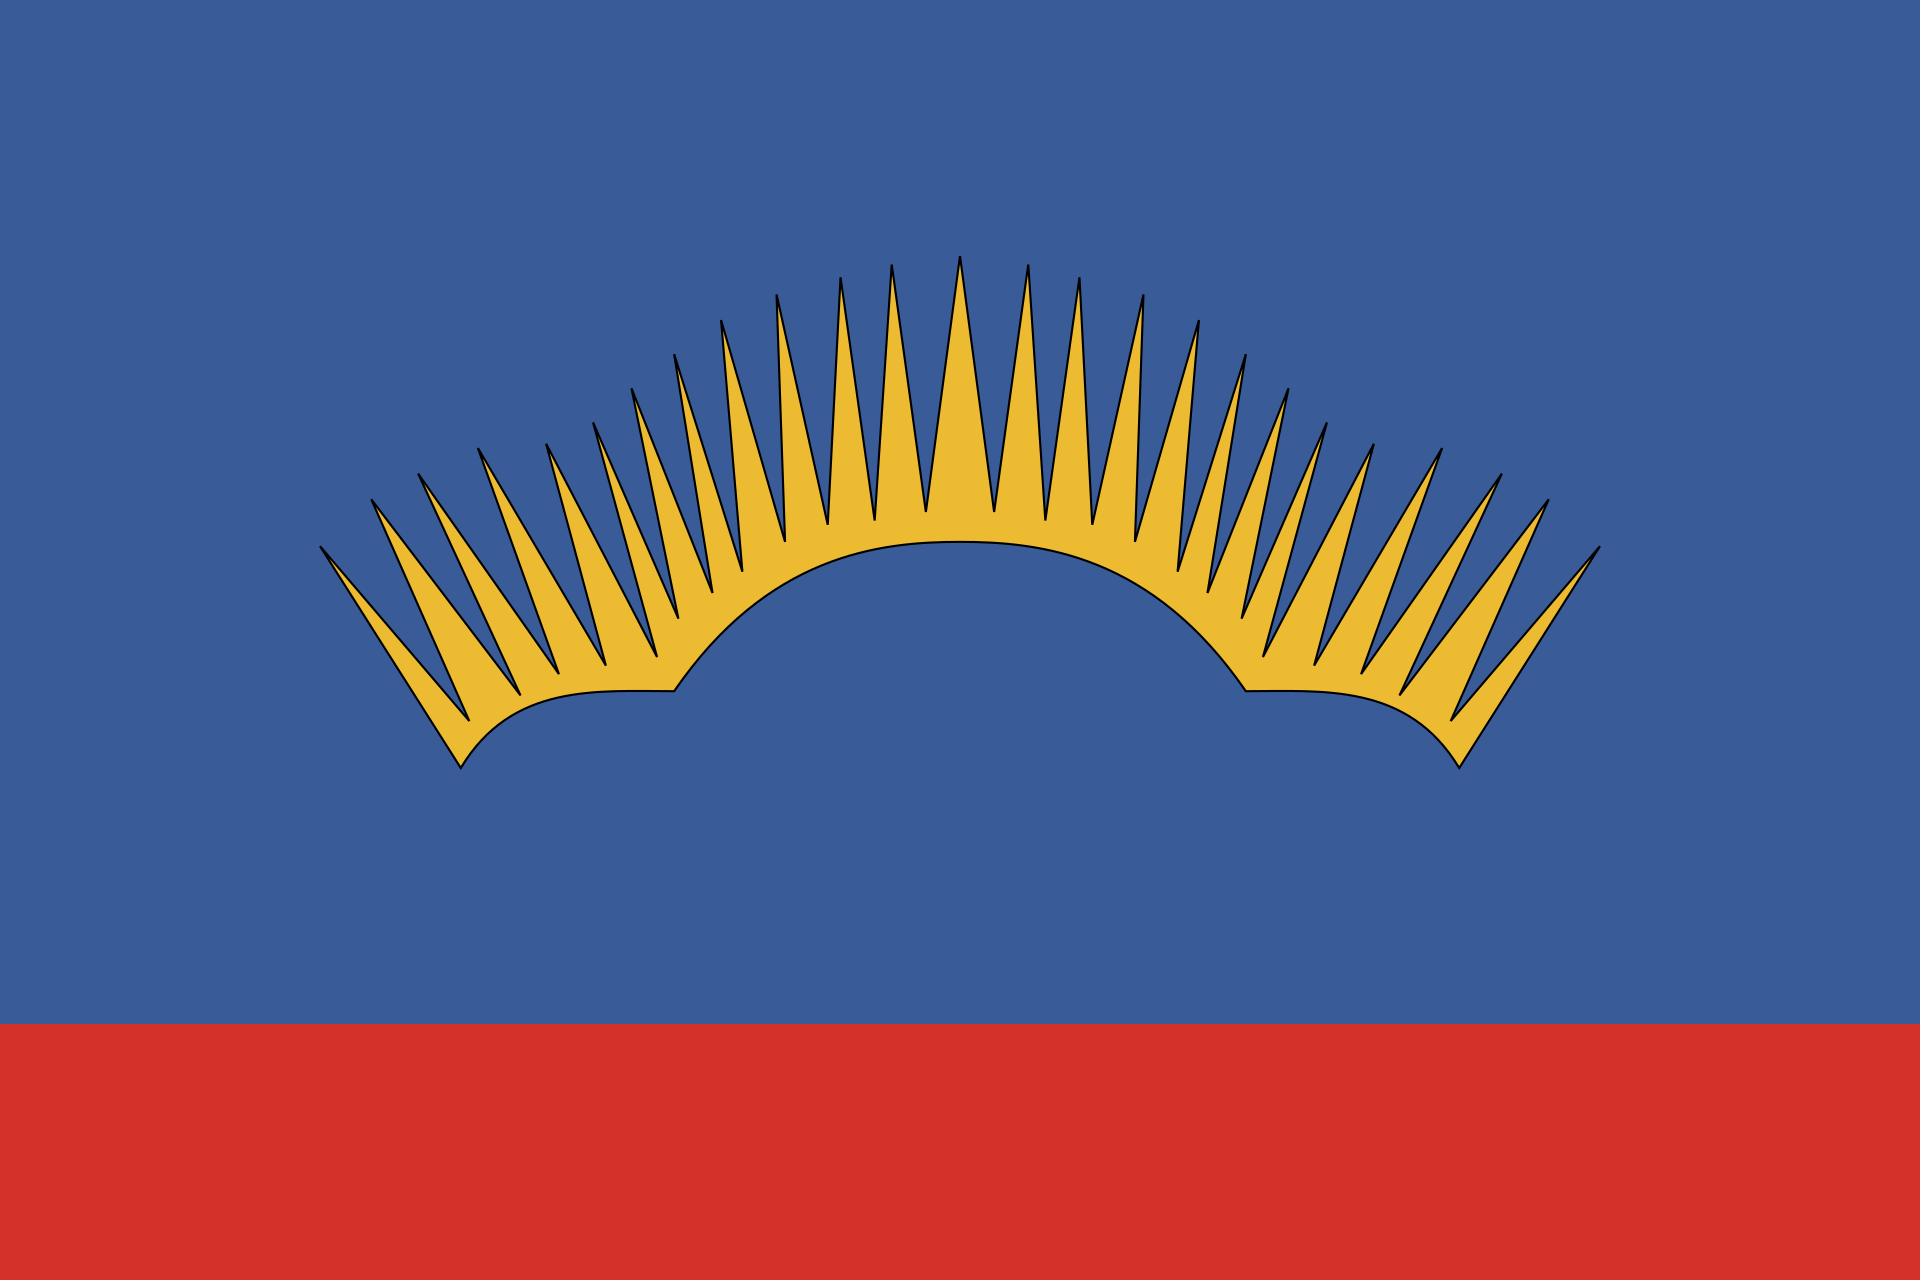
\includegraphics[width=3cm]{"chapter/oblast_of_Russia/Flag_of_Murmansk_Oblast.png"}
\caption [Флаг Мурманской области.]{Флаг Мурманской области.}%
\label{fig:Flag_of_Murmansk_Oblast}%
\end{marginfigure}


\lstset{numbers=left, firstnumber=1, frame=single}
\begin{lstlisting}[ language=SPARQL, 
                    caption=Граф соседних субъектов России\protect\footnotemark,
                    label=lst:sharesBorderWith-oblast-of-Russia,
                    texcl 
                    ]
# Graph of "subjects of Russia" `shares border with`. 
#defaultView:Graph
SELECT * WHERE 
{
  SERVICE wikibase:label { bd:serviceParam wikibase:language "ru"}
  { # no borders with the objects of Russia
    SELECT ?subject ?subjectLabel ?rgb ?subjects ?subjectsLabel WHERE
    {
      # Oblast, Republic, Federal city, Krai, Autonomus oblast, Autonomus okrug of Russia
      VALUES ?type {wd:Q835714 wd:Q41162 wd:Q183342 wd:Q831740 wd:Q309166 wd:Q184122}
      ?subject wdt:P31 ?type.  # instance of
    }
  }
  UNION  # Autonomus okrug of Russia
  { 
    SELECT ?subject ?subjectLabel ?rgb ?s ?sLabel WHERE
    {
      VALUES ?type {wd:Q835714 wd:Q41162 wd:Q183342 wd:Q831740 wd:Q309166 wd:Q184122}
      ?okrug wdt:P31 wd:Q184122; # is instance of Autonomus okrug of Russia
             wdt:P47 ?s.         # share border with ?s
                     ?s wdt:P31 ?type.
      BIND(IF(?okrug != '',"9932CC", IF(?rgb != '',?rgb,"FFFFFF")) AS ?rgb).
      BIND(IF(?okrug != '',?okrug, ?s) AS ?subject).
    }
  }
  UNION  # Autonomus oblast of Russia
  {
    SELECT ?subject ?subjectLabel ?rgb ?s ?sLabel WHERE
    {
      VALUES ?type {wd:Q835714 wd:Q41162 wd:Q183342 wd:Q831740 wd:Q309166 wd:Q184122}
      ?auto_oblast wdt:P31 wd:Q309166; # instance of Autonomus oblast of Russia
              wdt:P47 ?s.
                      ?s wdt:P31 ?type.
  
      BIND(IF(?auto_oblast != '',"ced685",IF(?rgb != '',?rgb,"FFFFFF")) AS ?rgb).
      BIND(IF(?auto_oblast != '',?auto_oblast, ?s) AS ?subject).
    }
  }
  UNION  # Krai of Russia
  {
    SELECT ?subject ?subjectLabel ?rgb ?s ?sLabel WHERE
    {
      VALUES ?type {wd:Q835714 wd:Q41162 wd:Q183342 wd:Q831740 wd:Q309166 wd:Q184122}
      ?krai wdt:P31 wd:Q831740; # instance of Krai of Russia
            wdt:P47 ?s.
                    ?s wdt:P31 ?type.
      BIND(IF(?krai != '',"7495db",IF(?rgb != '',?rgb,"FFFFFF")) AS ?rgb).
      BIND(IF(?krai != '',?krai, ?s) AS ?subject).
    }
  }
  UNION  # Federal city of Russia
  {
    SELECT ?subject ?subjectLabel ?rgb ?s ?sLabel WHERE
    {
      VALUES ?type {wd:Q835714 wd:Q41162 wd:Q183342 wd:Q831740 wd:Q309166 wd:Q184122}
      ?fed_city wdt:P31 wd:Q183342; # instance of Federal city of Russia
            wdt:P47 ?s.
                    ?s wdt:P31 ?type.
      BIND(IF(?fed_city != '',"e8a2e8",IF(?rgb != '',?rgb,"FFFFFF")) AS ?rgb).
      BIND(IF(?fed_city != '',?fed_city, ?s) AS ?subject).
    }
  }
  UNION  # Republic of Russia
  {
    SELECT ?subject ?subjectLabel ?rgb ?s ?sLabel WHERE
    {
      VALUES ?type {wd:Q835714 wd:Q41162 wd:Q183342 wd:Q831740 wd:Q309166 wd:Q184122}
      ?republic wdt:P31 wd:Q41162; # instance of Republic of Russia
                wdt:P47 ?s.
                        ?s wdt:P31 ?type.
      BIND(IF(?republic != '',"7FFF00",IF(?rgb != '',?rgb,"FFFFFF")) AS ?rgb).
      BIND(IF(?republic != '',?republic, ?s) AS ?subject).
    }
  }
  UNION  # Oblast of Russia
  {
    SELECT ?subject ?subjectLabel ?rgb ?s ?sLabel WHERE
    {
      VALUES ?type {wd:Q835714 wd:Q41162 wd:Q183342 wd:Q831740 wd:Q309166 wd:Q184122}
      ?oblast wdt:P31 wd:Q835714; # instance of Oblasts of Russia
              wdt:P47 ?s.
                      ?s wdt:P31 ?type.
      BIND(IF(?oblast != '',"e87b7b",IF(?rgb != '',?rgb,"FFFFFF")) AS ?rgb).
      BIND(IF(?oblast != '',?oblast, ?s) AS ?subject).
    }
  }
}
\end{lstlisting}%
\footnotetext[3][-14\baselineskip]{Получено 467 записей в 2017 году 
и 482 записи в 2021 году. Ссылку на~SPARQL-запрос не приводим из-за её чрезмерной длины. 
Вот ссылка на исходный запрос (\url{https://w.wiki/4DKD}), 
от которого мы отталкивались для построения этого мега запроса. 
Подумайте, как можно сократить или свернуть этот огромный запрос, сделать его компактным и элегантным?%
}
%
%
\begin{marginfigure}[1\baselineskip]
	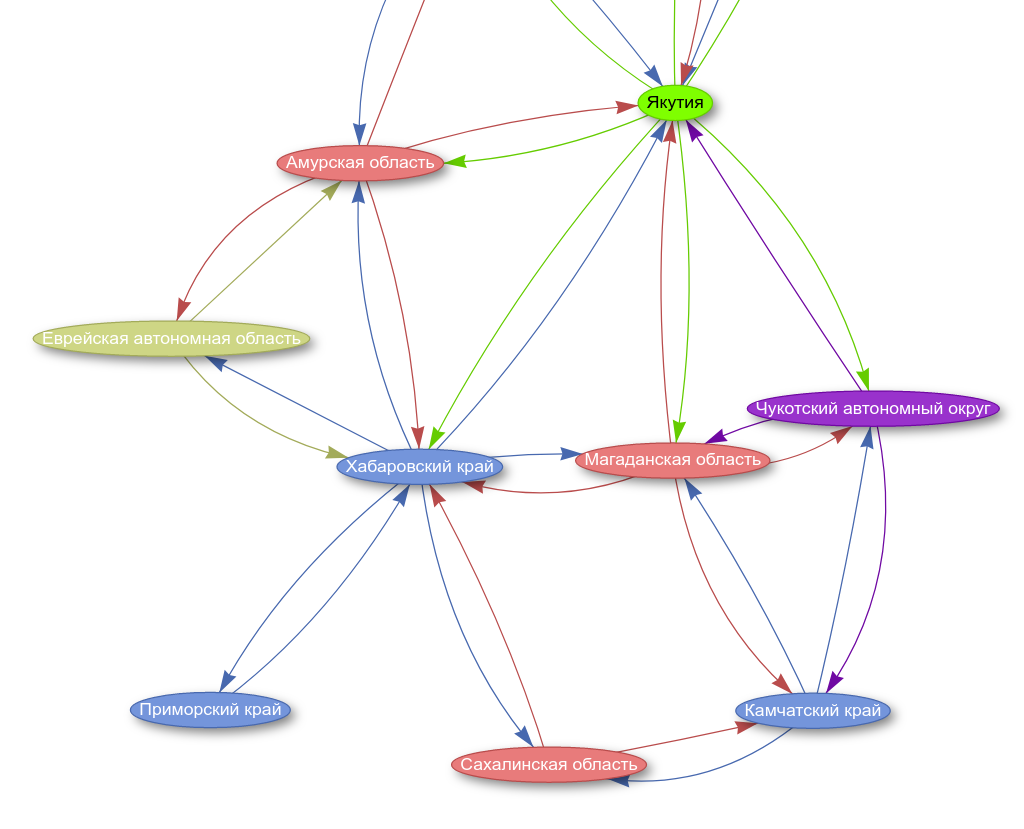
\includegraphics[width=1\textwidth]{./chapter/oblast_of_Russia/Graph_Subjects_of_Russia_Siberia_and_the_Far_East_2021.png}
	\caption[Фрагмент графа субъектов России, 2021 год.]{Регионы России в Сибире и Дальнем востоке на~2021 год. 
    Фрагмент графа соседних субъектов России, построенный по скрипту~\protect\ref{lst:sharesBorderWith-oblast-of-Russia}.
	Республики~--- вершины зелёного цвета (Якутия).
	Автономные округа~--- вершины фиолетового цвета (Чукотский автономный округ).
	Края~--- вершины голубого цвета (Хабаровский край).
	Области~--- вершины розового цвета (Амурская область).
	Автономные области~--- вершины салатового цвета (Еврейская автономная область).}%
      \label{fig:sharesBorderWith-oblast-of-Russia-Kaliningrad-fig}%
\end{marginfigure}


%\marginnote[-15\baselineskip]{
С помощью команды \lstinline|BIND| (строки 83--84) 
записываем значения в~переменные \lstinline|?rgb| и~\mbox{\lstinline|?subject|}, 
при условии, что эти переменные были пустыми. 

Переменная \lstinline|?oblast| ищется в строках 80--82. 
Подбирается такой объект \lstinline|?oblast|, 
который одновременно является 
экземпляром объекта \wdqName{<<области России>>}{835714} 
и~\wdProperty{47}{<<граничит~с>>}~объектом~\lstinline|?s|. 
При этом переменная \lstinline|?s| является экземпляром какого-либо типа субъектов РФ 
(то есть \lstinline|?s|~--- это экземпляр переменной \lstinline|?type|, 
заданной в~виде списка в~строке~79).

Если найдена переменная \lstinline|?oblast|, 
соответствующая условиям строк 80--82, 
тогда, во-первых, присваиваем \lstinline|?subject := ?oblast| (строка~84). 
Во-вторых, если к~тому~же переменная \lstinline|?rgb| ещё пуста, 
то присваиваем розовый цвет переменной \lstinline|?rgb := "e87b7b"| (строка~83). 
Этот цвет на рис.~\protect~\ref{fig:sharesBorderWith-oblast-of-Russia-Kaliningrad-fig} 
соответствует трём областям: Амурской, Магаданской и Сахалинской. 

Если переменная \lstinline|?oblast| уже не~пустая, а~цвет ещё не~задан, 
то выбираем светло-серый цвет \lstinline|?rgb := "FFFFFF"| (строка~83).
Если переменная \lstinline|?oblast| найдена, а цвет \lstinline|?rgb| уже задан, 
то мы его оставляем, то есть перезаписываем \lstinline|?rgb := ?rgb|.
%}

Количество полученных записей формируется путём сложения количества соседних территорий для всех субъектов России. 
Результат работы скрипта~--- это граф, 
отображающий соседние субъекты. 
Причём разные типы субъектов имеют вершины разного цвета, например, 
республики~--- зелёные, а края~--- голубые. 
Часть графа представлена на рис.~\ref{fig:sharesBorderWith-oblast-of-Russia-Kaliningrad-fig}.%




\newpage
Построим карту, на которой цветом обозначены субъекты России, 
граничащие с зарубежными странами. 
Более тёмным цветом обозначены субъекты, у которых большее количество пограничных стран, 
более светлым~--- с меньшим количеством пограничных стран (листинг~\ref{lst:sharesBorderWith-subjects-of-Russia}).

Результат работы запроса~\ref{lst:sharesBorderWith-subjects-of-Russia} 
представлен на рис.~\ref{fig:MapsharesBorderWithsubjectsofRussia}.


%\begin{fullwidth}
\begin{marginfigure}
	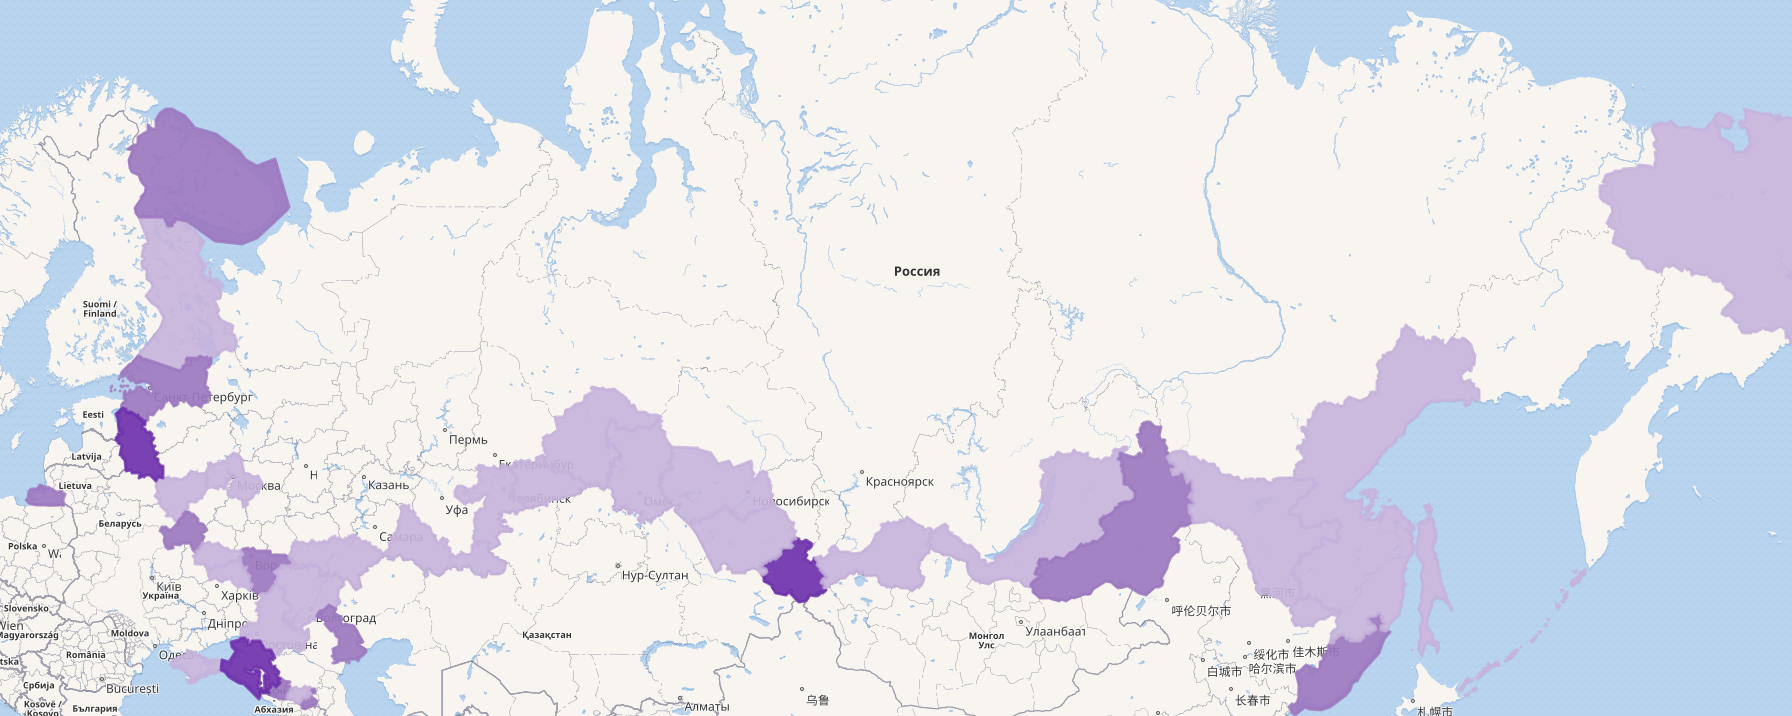
\includegraphics[width=\textwidth]{./chapter/oblast_of_Russia/Maps_of_the_subjects_of_Russia.png}
	\caption[Карта пограничных субъектов России, 2021 год.]{Карта субъектов России, граничащих с зарубежными странами, 2021 год. Карта построена с помощью запроса~\protect\ref{lst:sharesBorderWith-subjects-of-Russia}.}%
      \label{fig:MapsharesBorderWithsubjectsofRussia}%
\end{marginfigure}
%\end{fullwidth}

\lstset{numbers=left, firstnumber=1, frame=single}
\begin{lstlisting}[ language=SPARQL, 
                    caption={\href{https://w.wiki/4e82}{Карта субъектов России, граничащих с зарубежными странами}\protect\footnotemark},
                    label=lst:sharesBorderWith-subjects-of-Russia,
                    texcl 
                    ]
# Map of countries around Russia with the number of neighboring regions of Russia
#defaultView:Map\{"hide":["?shape", "?rgb"], "layer": "?regionLabel" \}
SELECT ?region ?regionLabel ?count ?shape ?rgb
{
  {
    SELECT ?region (COUNT(DISTINCT ?country) AS ?count) WHERE {
      VALUES ?type {
        wd:Q835714  # oblasts of Russia - 9 neighbours
        wd:Q41162   # republic of Russia - 4
        wd:Q183342  # federal city of Russia - 0 neighbours
        wd:Q831740  # krai of Russia - 4
        wd:Q309166  # autonomous oblast of Russia - 1
        wd:Q184122   # autonomous okrug of Russia - 1
      }
      ?region wdt:P31 ?type.
  
      # Russian region share border with some territory 
      # of foreign country
      ?region wdt:P47 [ wdt:P17 ?country].
      FILTER (?country != wd:Q159) # foreign country is not Russia
    }
    GROUP BY ?region HAVING ((COUNT(?country)) > 0)
  }
  ?region wdt:P3896 ?shape.
  BIND(IF(?count = 3 , "6c2eab", 
            IF(?count = 2 , "9b77bf", 
                IF(?count = 1 , "c6b2db", "f5cbce"))) AS ?rgb)
  SERVICE wikibase:label { bd:serviceParam wikibase:language "ru" }  
}
\end{lstlisting}%
\footnotetext{Получено 37 записей в 2021 году. SPARQL-запрос: \href{https://w.wiki/4e82}{https://w.wiki/4e82}}




Построим карту (рис.~\ref{fig:MapsoftheneighbouringstatesofRussia}), 
на которой цветом обозначены зарубежные страны, 
граничащие с субъектами России. 
Более тёмным цветом обозначены страны, у которых большее количество пограничных субъектов России, 
более светлым~--- с меньшим количеством пограничных субъектов России 
(запрос~\ref{lst:Maps_of_the_neighbouring_states_of_Russia}).
%
%\begin{fullwidth}
%\begin{figure}[h]
\begin{marginfigure}[0\baselineskip]
	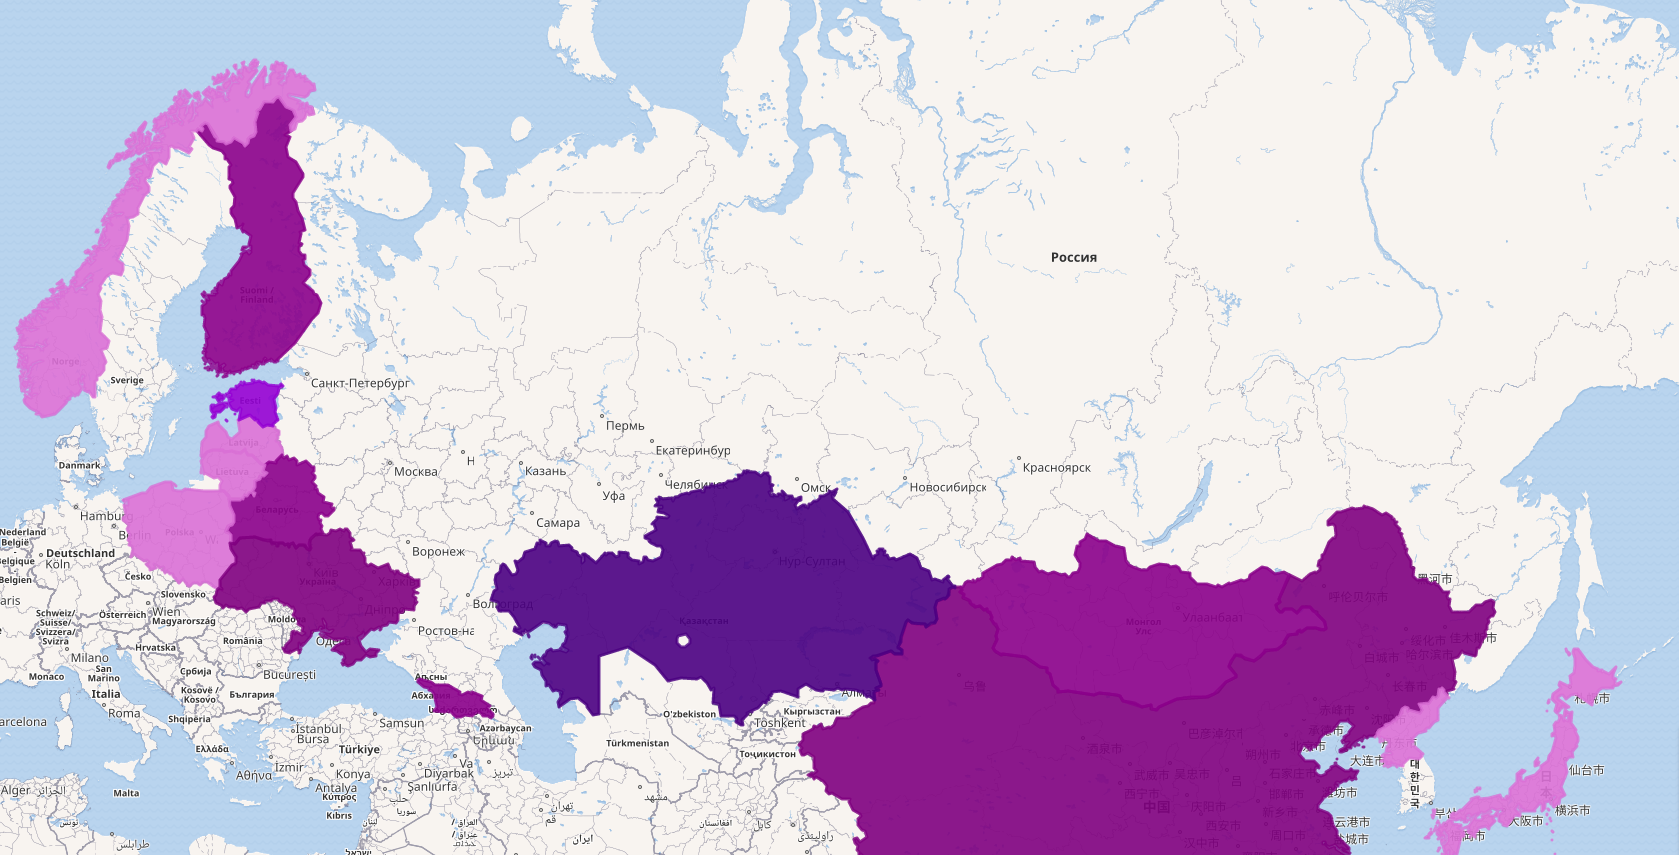
\includegraphics[width=\textwidth]{./chapter/oblast_of_Russia/Maps_of_the_neighbouring_states_of_Russia.png}
	\caption[Карта стран, граничащих с Россией, 2021 год.]{Карта стран, граничащих с субъектами России, 2021. Карта построена с помощью запроса~\protect\ref{lst:Maps_of_the_neighbouring_states_of_Russia}.}%
      \label{fig:MapsoftheneighbouringstatesofRussia}%
\end{marginfigure} 
%\end{fullwidth}

\lstset{numbers=left, firstnumber=1, frame=single}
\begin{lstlisting}[ language=SPARQL, 
                    caption={\href{https://w.wiki/4e8T}{Карта стран, граничащих с субъектами России}\protect\footnotemark},
                    label=lst:Maps_of_the_neighbouring_states_of_Russia,
                    texcl 
                    ]
# Map of countries around Russia with the number of neighboring regions of Russia
#defaultView:Map\{"hide":["?shape", "?rgb"], "layer": "?countryLabel"\}
SELECT ?country ?countryLabel ?count ?shape ?rgb WHERE {
{
    SELECT ?country (COUNT(DISTINCT ?region) AS ?count) WHERE {
      VALUES ?type {wd:Q835714 wd:Q41162 wd:Q183342 wd:Q831740 wd:Q309166 wd:Q184122}
      ?region wdt:P31 ?type;
              wdt:P47 [wdt:P17 ?country].
      FILTER (?country != wd:Q159) # foreign country is not Russia
    }
    GROUP BY ?country HAVING ((COUNT(?region)) > 0)
  }
  ?country wdt:P3896 ?shape.
  BIND(IF(?count > 9 , "4B0082", 
        IF(?count > 5 , "800080", 
         IF(?count > 2 , "8B008B", 
          IF(?count > 1 , "9400D3", 
           IF(?count > 0 , "DA70D6", "f5cbce"))))) AS ?rgb)
  SERVICE wikibase:label {bd:serviceParam wikibase:language "ru".}
}
\end{lstlisting}%
\footnotetext{Получено 15 записей в 2021 году. 
SPARQL-запрос: \href{https://w.wiki/4e8T}{https://w.wiki/4e8T}}




\newpage
\subsection{Полнота Викиданных}

С помощью запроса~\ref{lst:sharesBorderWith-empty-oblast-of-Russia} 
построим список субъектов России 
с~пустым свойством \wdProperty{47}{``shares border with''} (граничит с), 
то есть попробуем найти такие субъекты, которые ни с кем не граничат.

\label{question:q_subjects_of_Russia_2}
\marginnote{Какие из перечисленных далее субъектов входят в состав Российской Федерации, а какие~--- нет:
\begin{itemize}
  \item Республика Адыгея;
  \item Камчатский край;
  \item Читинская область;
  \item Чукотский автономный округ.
\end{itemize}
См. ответ \ref{answer:subjects_of_Russia_2} на с.~\pageref{answer:subjects_of_Russia_2}.
}


С помощью команды \lstinline|FILTER| (строка 15 запроса~\ref{lst:sharesBorderWith-empty-oblast-of-Russia}) 
исключаем объекты, которые не~находятся на территории России. 
Затем с помощью команды \lstinline|MINUS| (строка 18) удаляем из рассмотрения объекты, 
у которых свойство \wdProperty{47}{<<граничит с>>} заполнено.

Таким образом, на Викиданных для всех субъектов России свойство \wdProperty{47}{<<граничит с>>} заполнено.

%\marginnote[4.0cm]{Получено 0 записей в 2017 и 2021 годах. SPARQL-запрос: \href{https://w.wiki/5CHV}{https://w.wiki/5CHV}}
\lstset{numbers=left, firstnumber=1, frame=single}
\begin{lstlisting}[ language=SPARQL, 
                    caption={\href{https://w.wiki/5CHV}{Список субъектов РФ с пустым свойством \wdProperty{47}{``shares border with''}}\protect\footnotemark},
                    label=lst:sharesBorderWith-empty-oblast-of-Russia,
                    texcl 
                    ]
# List of `subjects of Russia` without `shares border with`. 
SELECT 
    ?subject ?subjectLabel 
    ?sharesBorderWith ?sharesBorderWithLabel
WHERE
{
  VALUES ?type {wd:Q835714   # Oblast of Russia
                wd:Q41162    # Republic of Russia
                wd:Q183342   # Federal city of Russia
                wd:Q831740   # Krai of Russia
                wd:Q309166   # Autonomus oblast of Russia
                wd:Q184122}  # Autonomus okrug of Russia
  ?subject wdt:P31 ?type.
  
  FILTER EXISTS {?subject wdt:P17 wd:Q159; 
                          wdt:P31 ?type}
  
  MINUS { ?subject  wdt:P47 [] }. # shares border with 
  SERVICE wikibase:label { bd:serviceParam wikibase:language "ru"}
}
\end{lstlisting}%
\footnotetext{Получено 0 записей в 2017 и 2021 годах. SPARQL-запрос: \href{https://w.wiki/5CHV}{https://w.wiki/5CHV}}




\section{Численность населения по субъектам Российской Федерации}

Обозначим на карте субъекты Российской Федерации, 
разделив их на шесть групп по количеству населения. 
Субъектам, принадлежащим одной группе, будет соответствовать на карте один цвет.

Для запроса~\ref{lst:population-map-of-Russia} нам потребуются свойства \wdProperty{625}{<<координаты>>} 
и \wdProperty{1082}{<<численность населения>>}.

\index{График!Map!Карта населения России}
\begin{lstlisting}[ language=SPARQL, numbers=none,
                    caption={\href{https://w.wiki/4bHe}{Карта населения России}\protect\footnotemark},
                    label=lst:population-map-of-Russia,
                    texcl 
                    ]
# Map of population of subjects of Russia
#defaultView:Map
SELECT DISTINCT ?subject ?subjectLabel ?population ?coord ?layer
{
  {
    { ?subject wdt:P31 wd:Q835714 } UNION  # Oblast of Russia
    { ?subject wdt:P31 wd:Q41162 } UNION  # Republic of Russia
    { ?subject wdt:P31 wd:Q183342 } UNION  # Federal city of Russia
    { ?subject wdt:P31 wd:Q831740 } UNION  # Krai of Russia
    { ?subject wdt:P31 wd:Q309166 } UNION # Autonomus oblast 
                                                        of Russia
    { ?subject wdt:P31 wd:Q184122 } # Autonomus okrug of Russia
  }   
  ?subject wdt:P625 ?coord; wdt:P1082 ?population.
  
  BIND(
    IF(?population < 500000, "< 500000",
    IF(?population < 1000000, "500000 - 1000000",
    IF(?population < 3000000, "1000000 - 3000000",
    IF(?population < 8000000, "3000000 - 8000000",
    IF(?population < 10000000, "8000000 - 10000000",
    "> 10000000")))))
    AS ?layer).
  
  SERVICE wikibase:label { bd:serviceParam wikibase:language "ru"}
}
ORDER BY ?population
\end{lstlisting}%
\footnotetext{Получено \num{85} записей в 2017 году и \num{86} записей в 2021 году. Ссылка на SPARQL-запрос: \href{https://w.wiki/4bHe}{https://w.wiki/4bHe}}

Результат работы запроса~\ref{lst:population-map-of-Russia} представлен на рис.~\ref{fig:SubjectsRussiaMap}.

\begin{fullwidth}
\begin{figure*}[h]
	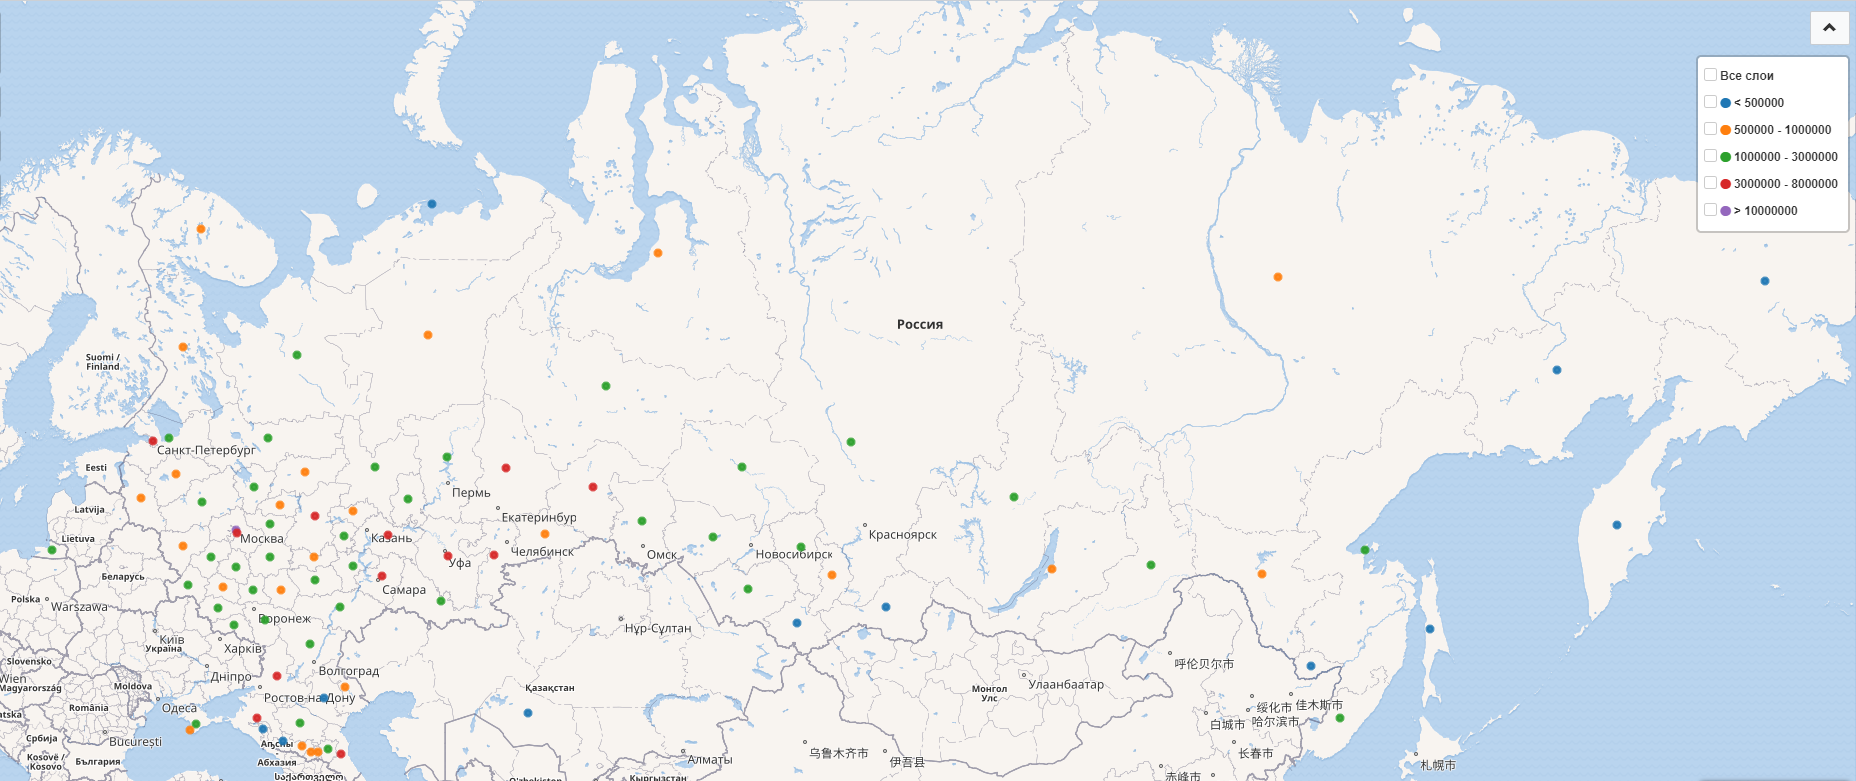
\includegraphics[width=\textwidth]{./chapter/oblast_of_Russia/SubjectsRussia_Map_with_legend_RU.png}
	\caption[Карта численности населения по субъектам России, 2021 год.]{Карта численности населения по субъектам России, 2021 год. Субъекты разделёны на шесть групп по количеству населения и отмечены разными цветами в зависимости от группы, в которую субъект входит. Карта построена с~помощью запроса~\protect\ref{lst:population-map-of-Russia}.}%
      \label{fig:SubjectsRussiaMap}%
\end{figure*} 
\end{fullwidth}

